% !TeX spellcheck = ru_RU
% !TeX root = lambda2024.tex


\newcommand{\tb}[1]{\textcolor{blue}{#1}}
\newcommand{\tr}[1]{\textcolor{red}{#1}}

\begin{frame}{Введение: $\lambda$-исчисление}
  \begin{figure}
    \centering
    \begin{subfigure}[t]{0.45\textwidth}
      \begin{minipage}{0.7\textwidth}
      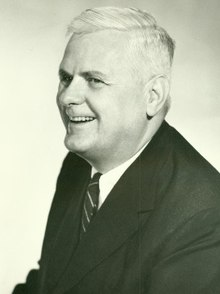
\includegraphics[width=1\textwidth]{220px-Alonzo_Church.jpg}\\
            Алонзо Чёрч (1903--1995)
      \end{minipage}
    \end{subfigure}
    \begin{subfigure}[t]{0.45\textwidth}
      \vspace{-5em}   % TODO: dirty hack!
  Алонзо Чёрч в 1935   открыл $\lambda$-исчисление
\vspace{1em}

Аналогичный подход от А.~Тьюринга с его машинами Тьюринга
\vspace{1em}

Это разные подходы для формализации понятия \enquote{алгоритм}
\vspace{1em}

В принципе, могло быть изобретено уже в 1910-х г.г.
\footnotetext{Изображение из \href{https://en.wikipedia.org/wiki/Alonzo\_Church}{Википедии}}

    \end{subfigure}
  \end{figure}
\end{frame}

\begin{frame}{Для формализации алгоритмов}
$\lambda$-исчисление можно использовать как формализацию понятия \enquote{алгоритм}

\begin{definition}[Алгоритм (неформально)]
Это конечная последовательность действий (или операций), к которым относятся все компьютерные программы, бюрократические процедуры, кулинарные рецепты и т.п.
\end{definition}

Алгоритмы, которые иногда дают ответ, а иногда не завершаются, называются \textit{разрешающими процедурами}.
\end{frame}

\begin{frame}{Проблемы неформального определения}
Зависимо от естественного языка\\


\vspace{1em}
Не совсем понятно, что является допустимой операцией, а что нет.
\begin{itemize}
    \item \enquote{Возьмите два любых решения уравнения $a^n+b^n=c^n$, для $n>2$ и $a,b,c\in \mathcal{N}$...}
	\item \enquote{Если это утверждение ложно, то ...}
	\item \enquote{Объявим как $A$ множество всех множеств. Если $A\in A$, то делаем одно, иначе --- другое}
\end{itemize}
\end{frame}


\begin{frame}{Зачем формализовывать то, что и так понятно?}
\framesubtitle{\enquote{Наивная} теория множеств}
 	\begin{figure}[t]
 		\begin{subfigure}[t]{0.60\textwidth}
 			\vspace{-7em}
% 			Множества можно делить на два типа
% 			\begin{enumerate}
% 				\item   набор не является элементом самого себя
% 				\item Расселовские: набор является элементом самого себя.
% 			\end{enumerate}
 			Рассмотрим $P=\{y: y\notin P\}$ и задумаемся про $P\in P$?
 			\begin{itemize}
 				\item Если формула верна, то нарушается определение
 				\item Если ложна, то не принадлежит, но по определению должна
 			\end{itemize}
 			\footnotetext{Изображение из \href{https://en.wikipedia.org/wiki/Bertrand\_Russell}{Википедии}}

 		\end{subfigure}
 		\hspace{0.05\textwidth}
 		\begin{subfigure}[t]{0.30\textwidth}
 			\begin{minipage}{0.7\textwidth}
 				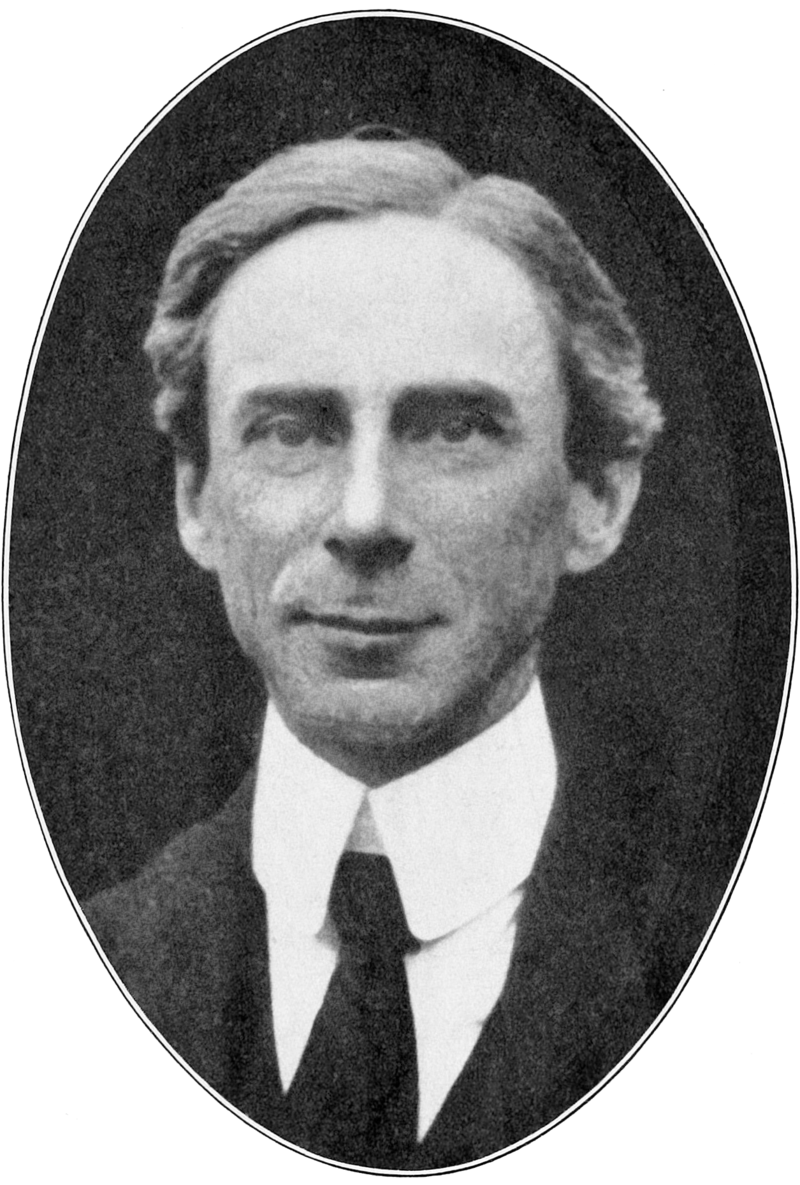
\includegraphics[width=1\textwidth]{800px-Bertrand_Russell_transparent_bg.png}\\
 				\centering
 				Bertrand~Russell \\(1872--1970)
 			\end{minipage}
 		\end{subfigure}
 	\end{figure}
\end{frame}

\begin{frame}{Цель формализации}
Придумать набор недвусмысленных правил, таких что обычный офисный бюрократ (читайте, компьютер) мог им следовать и получать ожидаемый результат.\\

\vspace{1em}
Существуют много различных формализаций:
\begin{itemize}
\item $\lambda$-исчисление
\item Машины Тьюринга\footnote{Мало имеют общего с компьютерами. Считать А.Тьюринга изобретателем компьютеров~--- неправильно}
\item Машины Поста
\item Частично (объявленные) рекурсивные функции (англ. partial recursive function)
\item Алгорифмы Маркова
\end{itemize}
\end{frame}


\begin{frame}{Вывод из формализации в современности}
Всё, что соответствует формальному описанию алгоритма, можно запрограммировать на компьютере

\begin{definition}[Тезис Чёрча-Тьюринга]
Алгоритмом является всё то, что можно записать и исполнить в $\lambda$-исчислении (машине Тьюринга), с точностью до представления данных. И ничего более.
\end{definition}

\end{frame}


\begin{frame}{$\lambda$-исчисление}
Процессом вычислений является переписывание программы ($\lambda$-выражения, $\lambda$-терма) на бесконечном листе бумаги.

\vspace{1em}
Программы конечны и состоят из символов следующего вида.
\begin{enumerate}
\item Переменные, в слайдах будем их обозначать строчными латинскими буквами
\item Скобки закрывающиеся \texttt{)} и открывающиеся \texttt{(}
\item Точка как разделитель
\item Символ $\lambda$
\end{enumerate}
\end{frame}


\begin{frame}{$\lambda$-исчисление}
\begin{figure}[t]
  \begin{subfigure}[t]{0.35\textwidth}
    \vspace{-5em}
    \vspace{-1em}
    Синтаксис:
    \begin{itemize}
      \item Переменные: $x,y,z,\dots$
      \item Абстракция $(\lambda \nu. A)$, где \\
      $A$ --- $\lambda$-выражение, \\
      а $\nu$ --- произвольное имя переменной
      \item Применение $(AB)$, где $A$ и $B$ --- $\lambda$-выражения
      \item Ничего больше нет
    \end{itemize}
%    \begin{definition}{Редекс}
%      --- это $\lambda$-выражение вида $(\lambda \nu. A)B$
%    \end{definition}
  \end{subfigure}
\hspace{1cm}
  \begin{subfigure}[t]{0.55\textwidth}

      \vspace{-5.5em}
В терминах программирования:
\begin{itemize}
  \item Переменные
  \item Объявления 1-аргументных функций
  \item Вызов функции от одного аргумента
\end{itemize}
%    \vspace{1em}
%Процесс вычисления --- это процеcc устранения редексов (возможно, не всех) путём подстановок $\lambda$-выражений вместо переменных.
\end{subfigure}
\end{figure}
\end{frame}

\begin{frame}{Каррирование}
\begin{figure}[t]
  \begin{subfigure}[t]{0.4 \textwidth}
        \vspace{-10em}
\begin{definition}[Каррирование]
представление n-арных функций через 1-арные функции
\end{definition}

\vspace{1em}

В $\lambda$-исчислении функция $n$ аргументов представляются как функция одного аргумента, которые возвращает функцию от $n-1$ аргумента.\\

В мире названо в честь Хаскеля Карри. Впервые появилось в 1924 в работе М.~И.~Шейнфинкеля.\\

\footnotetext{Изображение взято с \href{https://en.wikipedia.org/wiki/Moses\_Sch\%C3\%B6nfinkel}{Википедии}}

  \end{subfigure}
\hspace{1cm}
  \begin{subfigure}[t]{0.25\textwidth}
      \begin{minipage}{1\textwidth}
      %\vspace{-3mm}
      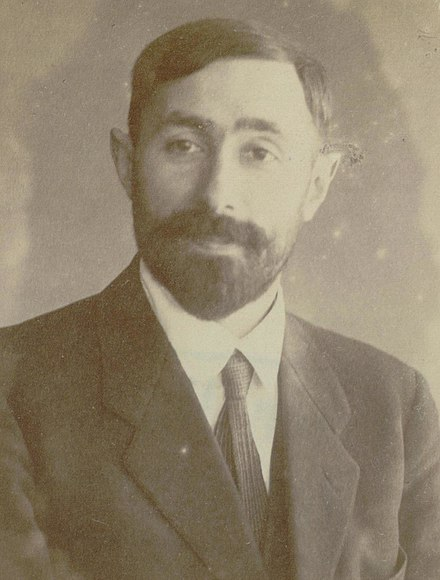
\includegraphics[width=1\textwidth]{440px-Moses_Schonfinkel_1922_(cropped).jpg}\\
      \centering      Моисей Исаевич Шейнфинкель \\(1888--1942)
    \end{minipage}
  \end{subfigure}
  \begin{subfigure}[t]{.25\textwidth}
    \begin{minipage}{1\textwidth}
      \vspace{-1mm}
      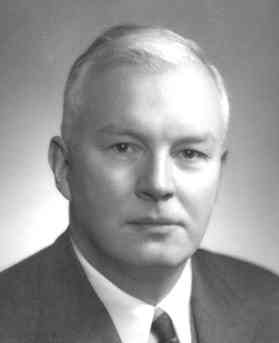
\includegraphics[width=1\textwidth]{Haskell_Curry.jpg}\\
      \centering Хаскел Карри \\(1900--1982)
    \end{minipage}
  \end{subfigure}
\end{figure}
\end{frame}



\begin{frame}[fragile]{Символ $\lambda$ работает как квантор}
  \tikzstyle{every picture}+=[remember picture]
  \tikzstyle{na} = [shape=rectangle,inner sep=0pt,text depth=0pt]
%  {\Large
%  \[
%  \lambda \tikz\node[na](dbI1){x}; . (\lambda \tikz\node[na](dbI2){z};.  \tikz\node[na](dbI3){x}; \tikz\node[na](dbI4){z};)  \tikz\node[na](dbI5){x};
%  \]
%  \begin{tikzpicture}[overlay]
%    \path[->,red,thick](dbI1) edge [out=90, in=90] (dbI3);
%    \path[->,red,thick](dbI1) edge [out=-90, in=-90] (dbI5);
%    \path[draw,->,blue,thick] (dbI2.south) -- ++(0,-0.2cm) -- ++(0.6cm,0) -- (dbI4.south);
%  \end{tikzpicture}
%}
  {\Large
  \[
  \lambda \tikz\node[na](dbM){m};.
  \lambda \tikz\node[na](dbN){n};.
  \lambda \tikz\node[na](dbF){f};.
  \lambda \tikz\node[na](dbX){x};.
  \app{\tikz\node[na](UM){m};\ \tikz\node[na](UF1){f};\ }{\app{\tikz\node[na](UN){n};\  \tikz\node[na](UF2){f};\ }{\tikz\node[na](UX){x};}}
  \]
  \begin{tikzpicture}[overlay]
    \path[->, red,thick](dbM) edge [out=90, in=90] (UM);
    \path[->,blue,thick](dbN) edge [out=90, in=90] (UN);
    \path[->, red,thick](dbF) edge [out=-90, in=-90] (UF1);
    \path[->, red,thick](dbF) edge [out=-90, in=-90] (UF2);
    \path[->, red,thick](dbX) edge [out=90, in=90] (UX);
%    \path[draw,->,blue,thick] (dbF.south) -- ++(0,-0.2cm) -- ++(0.6cm,0) -- (dbI4.south);
  \end{tikzpicture}
}
\begin{itemize}
  \item свободные вхождения
  \item связанные вхождения и т.д.
\end{itemize}

\footnotetext{TODO: сказать про скобочки}
\end{frame}


\begin{frame}[fragile]{Подстановка}
 \begin{figure}[t]
   \begin{subfigure}[t]{0.45\textwidth}
   \vspace{-5em}
    \begin{definition}[Редекс]
      $\lambda$-выражение вида $(\lambda x. B)A$
    \end{definition}

    \vspace{2em}
    Подстановка \enquote{$A$ вместо $x$ в выражении $B$} в лит-ре обозначается по-разному:
      \begin{itemize}
        \item \subst{x}{A}{B}
        \item \substt{x}{A}{B}
      \end{itemize}
      \vspace{1em}
      \[
          (\lambda x. B)A \xarr{\beta}    \subst{x}{A}{B}
      \]
   \end{subfigure}
   \hspace{1cm}
   \begin{subfigure}[t]{0.45\textwidth}
   \begin{minipage}{\textwidth}

Редекс $\lam{x}{\lam{x}{x} x}y$ вида $(\lambda \nu. B)A$, где
\begin{itemize}
  \item $B \equiv \lam{x}{x} x$
  \item $A \equiv  y$
  \item $\nu \equiv x$
\end{itemize}
  \tikzstyle{every picture}+=[remember picture]
  \tikzstyle{na} = [shape=rectangle,inner sep=0pt,text depth=0pt]
  {\Large
    \[
    (\lambda \tikz\node[na](dbI1){x}; .
      (\lambda \tikz\node[na](dbI2){x};.  \tikz\node[na](dbI3){x}; )
      \tikz\node[na](dbI5){x};)
    y    \arr \lam{x}{x}y
    \]
    \begin{tikzpicture}[overlay]
      \path[->,red,thick](dbI1) edge [out=-90, in=-90] (dbI5);%      \path[draw,->,blue,thick] (dbI2) edge [out=-90, in=-90] (dbI3);
      \path[draw,->,blue,thick] (dbI2.south) -- ++(0,-0.2cm) -- ++(0.4cm,0) -- (dbI3.south);
    \end{tikzpicture}
  }
   \end{minipage}
   \begin{definition}[Один шаг ($\beta$-)редукции]
   это избавление от редекса  $(\lambda x. B)A$ путём совершения подстановки $A$ вместо $x$ в выражении $B$
   \end{definition}
   \end{subfigure}
 \end{figure}
\end{frame}

\begin{frame}{Как происходят вычисления (редукция) $\lambda$-исчислении?}
\begin{definition}[Редукция]
Процесс постепенного избавления от редексов. Редукция $\equiv$ вычисление $\lambda$-выражения
\end{definition}

\begin{definition}[Стратегия]
  Порядок выбора редексов регламентирует стратегия. Ищем редексы $(\lambda x. B)A$
  \begin{itemize}
    \item Если редексов нет, то вычисление закончилось
    \item Если редексы есть, стратегия регламентирует какой на данном шаге редекс стоит $\beta$-редуцировать
    \item Или же, стратегия может сказать, что все редексы нужно оставить как есть, и выдать ответ
  \end{itemize}
\end{definition}
    %Стратегий бывает много разных
    %\begin{enumerate}
    %  \item Строгая стратегия call-by-value .    Для $(\lambda x. P)Q$ вычисляет $Q\cbv Q'$ и потом подставляет $Q'$ вместо $x$ в $P$.
    %  \item Ленивая стратегия call-by-name.   Для $(\lambda x. P)Q$ сразу подставляет $Q$ вместо $x$ в $P$.
    %  \item Обе стратегии оставляют абстракции и переменные как есть
    %\end{enumerate}
\end{frame}

\begin{comment}
\begin{frame}{Экстенсиональность}
Есть хорошая причина для произвольного $f$ считать выражение $\lam{x}{f\ x}$ и $f$ эквивалентными

\begin{align*}
\app{\lam{x}{f\ x}}{\xi} \betaarr \app{f}{\xi}
\end{align*}
\end{frame}
\end{comment}

\begin{frame}{Что нужно для представления алгоритмов?}
  \begin{itemize}
    \item Принимать входные данные
    \item Делать ветвления  в зависимости от входных данных
    \item Совершать некоторое количество однотипных действий в зависимости от входных данных (т.е. должны быть циклы или их аналог --- рекурсия)
    \begin{itemize}
\item       Чтобы понимать, сколько действий уже сделали нужны натуральные числа
    \end{itemize}
  \end{itemize}
\end{frame}

\begin{frame}{Историческое напоминание: числа Пеано}
\begin{figure}[ht]
  \begin{subfigure}[t]{.55\textwidth}
  \vspace{-8em}
  Первым ввёл аксиоматику арифметики в 1889 году. Натуральные числа определяются через \textbf{\enquote{базу}} и \textbf{\enquote{следующий}}\\

  \begin{enumerate}
  \item[1.] 0 --- натуральное число
  \item[6.] Для любого натурального $n$, $S(n)$ тоже натуральное. т.е. натуральные числа замкнуты относительно операции $S(\cdot)$
  \item [9.] Аксиома индукции.
  \end{enumerate}
  \footnotetext{
  \href{https://www.researchgate.net/publication/240358753\_Peano's\_axioms\_in\_their\_historical\_context}{Peano's axioms in their historical context}
  }

  \footnotetext{Изображение взято с \href{https://en.wikipedia.org/wiki/Moses\_Sch\%C3\%B6nfinkel}{Википедии}}
  \end{subfigure}
\hspace{1cm}
\begin{subfigure}[t]{.35\textwidth}
  \begin{minipage}{1\textwidth}
    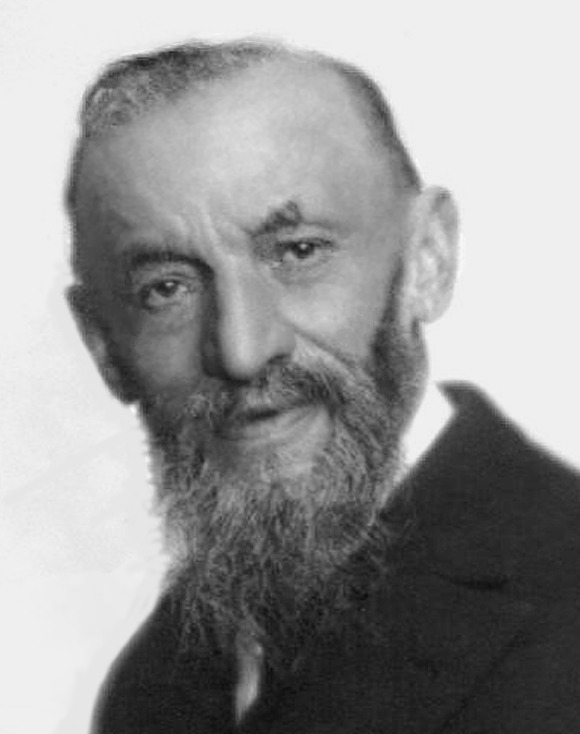
\includegraphics[width=1\textwidth]{Giuseppe_Peano.jpg}\\
    Джузеппе Пеано (1858--1932)
  \end{minipage}
\end{subfigure}
\end{figure}
\end{frame}


\defverbatim[colored]{\numeralIsFor}{
\begin{lstlisting}[language=c]
// Church numeral N
for (int i=0; i<N; i++)
  x = f(x);
\end{lstlisting}
}

\begin{frame}{Представление чисел (нумералы Чёрча). Сложение}
\begin{figure}[t]
    \begin{subfigure}[t]{0.45\textwidth}
$ 0 \sim \lam{f}{\lam{x}{\ x}}$

$ 1 \sim \lam{f}{\lam{x}{\ f\ x}}$

$ 2 \sim \lam{f}{\lam{x}{\ f\ (f\ x)}}$

  и т.д.
    \end{subfigure}
    \begin{subfigure}[t]{0.45\textwidth}
    \begin{minipage}{\textwidth}
    \numeralIsFor
    \end{minipage}
    \end{subfigure}
\end{figure}

  \vspace{1cm}

  Сложение (один из вариантов): взять два нумерала $m$ и $n$, взять $f$ и $x$, а затем к $x$ применить $f$ $n$ раз, а затем к результату применить $f$ $m$ раз.

\begin{align*}
add \equiv &\ \lam{m}{\lam{n}{\lam{f}{\lam{x}{\app{m\ f\ }{\app{n\ f\ }{x}}}}}}\\
\equiv &\ \lambda m. \lambda n. \lambda f. \lambda x. \app{m\ f\ }{\app{n\ f\ }{x}}
\end{align*}
\end{frame}


\begin{frame}{Вычисление (т.е. редукция, упрощение) 2+2}
\def\betaarr{\longrightarrow\!\!\beta}
\def\numTWO{\ensuremath{\lam{f}{\lam{x}{f(f\ x)}}}}
\vspace{-2em}
  \begin{align}
    \App{\lambda m. \lambda n. \lambda f. \lambda x. \app{m\ f\ }{\app{n\ f\ }{x}} }{2} 2 & \betaarr \\
    \Redex{(\lambda m. \lambda n. \lambda f. \lambda x. \app{m\ f\ }{\app{n\ f\ }{x}}) {}}{2} 2 & \betaarr \\
    \Redex{( \lambda n. \lambda f. \lambda x. \app{2\ f\ }{\app{n\ f\ }{x}}){}}{2} & \betaarr \\
    \lambda f. \lambda x. \app{2\ f\ }{\app{2\ f\ }{x}}   & \longrightarrow \\
    \lambda f. \lambda x. \App{\Redex{\numTWO}{f}\ }{\app{2\ f\ }{x}} & \betaarr \\
    \lambda f. \lambda x. \App{\lam{x}{f (f x)} \ \ }{\app{2\ f\ }{x}} & \longrightarrow \\
    \lambda f. \lambda x. \app{\lam{x}{f (f x)}} {\app{\App{\Redex{\numTWO}{f}}{x}}} & \betaarr \\
    \lambda f. \lambda x. \App{\lam{x}{f (f x)}  } {\Redex{\lam{x}{f (f x)} }{x}} & \betaarr \\
    \lambda f. \lambda x. \redex{\Lam{x}{f (f x)}}{\App{f}{\app{f}{x}}} & \betaarr \\
    \lambda f. \lambda x. f (f (f (f x))) & \equiv 4
  \end{align}
\end{frame}

\begin{frame}{Представление чисел (нумералы Чёрча). Умножение}
\begin{figure}[t]
    \begin{subfigure}[t]{0.45\textwidth}
$ 0 \sim \lam{f}{\lam{x}{\ x}}$

$ 1 \sim \lam{f}{\lam{x}{\ f\ x}}$

$ 2 \sim \lam{f}{\lam{x}{\ f\ (f\ x)}}$

  и т.д.
    \end{subfigure}
    \begin{subfigure}[t]{0.45\textwidth}
    \begin{minipage}{\textwidth}
    \numeralIsFor
    \end{minipage}
    \end{subfigure}
\end{figure}

  \vspace{1cm}


Умножение: взять два нумерала $m$ и $n$, взять $f$ и $x$, а затем к $x$ применить $n$ раз $f$, и повторить это $m$ раз.

\begin{align*}
mul \equiv &\ \lam{m}{\lam{n}{\lam{f}{\lam{x}{\app{\app{m}{\app{n\ f}}{\ x}}}}}}\\
\equiv &\ \lambda m. \lambda n. \lambda f. \lambda x. \app{\app{m}{\app{n\ f}}}{\ x} \\
%\simeq &\ \lambda m. \lambda n. \lambda f. \app{m}{\app{n\ f}} \\
\end{align*}
\end{frame}




%\begin{frame}{Вычисление (т.е. редукция, упрощение) 2$\times$2 без $\eta$-экспансии}
%\def\betaarr{\longrightarrow\!\!\beta}
%\setcounter{equation}{0}
%\vspace{-2em}
%\begin{align}
%  (\lam{m }{\lam{n}{\lam{z}{\app{m}{\app{n}{z}}}}} 2) 2  & \longrightarrow \\
%  \redex{\lam{m }{\lam{n}{\lam{z}{\app{m}{\app{n}{z}}}}}}{2} 2  & \betaarr \\
%  \redex{\lam{n}{\lam{z}{\app{2}{\app{n}{z}}}}}{2}  & \betaarr \\
%  \lam{z}{2 \app{2}{z}}  & \longrightarrow \\
%  \lam{z}{\tb{\lam{f}{\lam{x}{f(f\ x)}}} \textcolor{red}{\app{2}{z}}}  & \betaarr \\
%  \lam{z}{\lam{x}{\app{\app{2}{ z}}{(2\ z\ x)}}}  & \longrightarrow \\
%  \lam{z}{\lam{x}{\app{\app{\tb{\lam{f}{\lam{x}{f(f\ x)}}}}{\tr{z}}}{(2\ z\ x)}}}  & \betaarr \\
%    \lam{z}{\lam{x}{\textcolor{blue}{\lam{x}{\app{z}{\app{z}{x}}}} \tr{(2 z x)}}} & \betaarr \\
%  \lam{z}{\lam{x}{\app{z}{\app{z}{\app{\tb{2} \tr{z}}{x}}}}}  & \betaarr \\
%  \lam{z}{\lam{x}{\app{z}{\app{z}{\textcolor{blue}{\lam{x}{\app{z}{\app{z}{x}}}} \tr{x}}}}}  & \betaarr \\
%  \lam{z}{\lam{x}{\app{z}{\app{z}{\app{z}{\app{z}{x}}}}}} &  \equiv 4
%  \end{align}
%\end{frame}

\begin{frame}[plain]{Вычисление \\(т.е. редукция, упрощение) \\2$\times$2 длинно}
\def\betaarr{\longrightarrow\!\!\beta}
\def\numTWO{\ensuremath{\lam{f}{\lam{x}{f(f\ x)}}}}
\setcounter{equation}{0}
\begin{figure}[t]
  \begin{subfigure}[t]{0.35\textwidth}
  $\qquad$
  \end{subfigure}
  \begin{subfigure}[t]{0.55\textwidth}
        \vspace{-8em}
        \begin{align}
          \apppl{\app{\lam{m}{\lam{n}{\lam{z}{\lam{x}{(m \app{n}{z} x)}}}}}{2}}{2} & \longrightarrow \\
          \Apppl{\Redex{\lam{m}{\lam{n}{\lam{z}{\lam{x}{(m \app{n}{z} x)}}}}}{2}}{2} & \betaarr \\
          \Redex{\lam{n}{\lam{z}{\lam{x}{(2 \app{n}{z} x)}}}}{2} & \betaarr \\
          \lam{z}{\lam{x}{\app{\app{2}{\app{2}{z}}}{x}}} & \longrightarrow \\
          \lam{z}{\lam{x}{\App{\Redex{\numTWO}{\app{2}{z}}}{x}}} & \betaarr \\
          \lam{z}{\lam{x}{\Redex{\lam{x}{(2 z (2 z x))}}{x}}} & \betaarr \\
          \lam{z}{\lam{x}{\App{\app{2}{z}}{(2 z x)}}} & \longrightarrow \\
          \lam{z}{\lam{x}{\app{\Redex{\numTWO}{z}}{(2 z x)}}} & \betaarr \\
          \lam{z}{\lam{x}{\redex{\lam{x}{\app{z}{\app{z}{x}}}}{(2 z x)}}} & \betaarr \\
          \lam{z}{\lam{x}{\app{z}{\app{z}{\App{\app{2}{z}}{x}}}}} & \longrightarrow \\
          \lam{z}{\lam{x}{\app{z}{\app{z}{\App{\Redex{\numTWO}{z}}{x}}}}} & \betaarr \\
          \lam{z}{\lam{x}{\app{z}{\App{z}{\Redex{\lam{x}{\app{z}{\app{z}{x}}}}{x}}}}} & \betaarr \\
          \lam{z}{\lam{x}{\app{z}{\app{z}{\app{z}{\app{z}{x}}}}}} & \equiv 4
        \end{align}
  \end{subfigure}
\end{figure}

\end{frame}

\begin{comment}
\begin{frame}{Две стратегии: Call-by-value и аппликативная}
  \begin{figure}[t]
    \begin{subfigure}[t]{0.45\textwidth}
            \centering Call-by-value
      \begin{mathpar}
  \inferrule*  [Right=Abs] {\\}
{\lam{x}{e} \cbv \lam{x}{e}}
\end{mathpar}
    \end{subfigure}
    \begin{subfigure}[t]{0.45\textwidth}
      \centering
      Applicative order
      \begin{mathpar}
      \inferrule* [Right=Abs] {e \ao e'}
      {\lam{x}{e} \ao \lam{x}{e'}}
      \end{mathpar}
    \end{subfigure}
  \end{figure}
\hrulefill
\only<1>{
\begin{mathpar}
\inferrule*  [Right=App-abs]
{ f_1 \arr \lam{x}{e} \\
  a_1 \arr a_2 \\
  \subst{x}{a_2}{e} \arr r
}
{ (f_1 a_1) \arr r}
\end{mathpar}
\begin{mathpar}
  \inferrule* [Right=Var] {\\}
  {x \arr x}
  \and
  \inferrule*  [Right=App-non-abs]
{ f_1 \arr f_2 \neq \lam{x}{e} \\
  a_1 \arr a_2}
{ (f_1 a_1) \arr (f_2 a_2) }
\end{mathpar}
}
\only<2>{
\begin{figure}[t]
  \begin{subfigure}[t]{0.45\textwidth}
\begin{itemize}
\item[\faGood]    Подходит для написания произвольных алгоритмов
\vspace{4em}

\item[\faBad] Не считает под абстракцией, поэтому ответ иногда длиннее, чем хотелось бы
\end{itemize}
  \end{subfigure}
  \begin{subfigure}[t]{0.45\textwidth}
\begin{itemize}
  \item[\faBad] Нет возможности отложить вычисления на потом,т.е. в if-then-else вычисляется и then, и else. Нельзя дождаться ответа от рекурсивных функций
  \item[\faGood] Cчитает под абстракцией, поэтому ответ короче
\end{itemize}
  \end{subfigure}
\end{figure}
}
\end{frame}


\begin{frame}
\vspace{-1em}
\begin{mathpar}
\inferrule*  [Right=App-abs]
{ f_1 \arr \lam{x}{e} \\
  a_1 \arr a_2 \\
  \subst{x}{a_2}{e} \arr r
}
{ (f_1 a_1) \arr r}
\end{mathpar}
\begin{mathpar}
  \inferrule*  [Right=App-non-abs]
  { f_1 \arr f_2 \neq \lam{x}{e} \\
    a_1 \arr a_2}
  { (f_1 a_1) \arr (f_2 a_2) }
\end{mathpar}
\vspace{1em}

\cbvstrat
\end{frame}
\end{comment}

%\section{Написание алгоритмов с помощью лямбда-исчисления}



\begin{frame}{Ветвления}
\def\ite{\lam{c}{\lam{t}{\lam{e}{\ \app{\app{c}{t}}{e}}}}}
\[
T\equiv\lam{x}{\lam{y}{x}} \equiv f\!st \qquad \qquad \qquad \qquad
F\equiv \lam{x}{\lam{y}{y}}\equiv snd \equiv 0
\]

\begin{align*}
  ite \quad\equiv &\quad \lam{c}{\lam{t}{\lam{e}{\ \app{\app{c}{t}}{e}}}}\\
  (ite\ T) \quad\equiv &\quad \ite T \arrbeta \lambda t. \lambda e. (\app{T}{t}\ e) \arrmany \lam{t}{\lam{e}{t}}\equiv T\\
  (ite\ F) \quad\equiv &\quad \ite F \arrbeta \lambda t. \lambda e. (\app{F}{t}\ e) \arrmany \lam{t}{\lam{e}{e}}\equiv F
\end{align*}

%\footnotetext{
Здесь $\arrmany$ означает редукцию за несколько шагов
%}
\end{frame}




\begin{comment}

\begin{frame}{2+2}
  \begin{figure}[t]
    \begin{subfigure}[t]{0.50\textwidth}
      \begin{align*}
        (\lambda m. \lambda n. \lambda f. \lambda x. \app{m\ f\ }{\app{n\ f\ }{x}}){} 2 2 &\cbv \\
        \textcolor{blue}{(\lambda m. \lambda n. \lambda f. \lambda x. \app{m\ f\ }{\app{n\ f\ }{x}}) {}} \textcolor{red}{2} 2 &\cbv \\
        \textcolor{blue}{( \lambda n. \lambda f. \lambda x. \app{2\ f\ }{\app{n\ f\ }{x}}){}} \textcolor{red}{2} & \cbv \\
        \lambda f. \lambda x. \app{2\ f\ }{\app{2\ f\ }{x}}   &
      \end{align*}
      Это ответ для $\cbv$.\\

      Давайте посмотрим, что будет, если мы \\
      ответ применим к $g$ и $y$
    \end{subfigure}
    \begin{subfigure}[t]{0.45\textwidth}
      \begin{align*}
        (\lambda f. \lambda x. \app{2\ f\ }{\app{2\ f\ }{x}}) g y  &\arr \\
        (\lambda x. \app{2\ g\ }{\app{2\ g\ }{x}}) y  &\arr \\
        \app{2\ g\ }{\app{2\ g\ }{y}}   &\arr \\
        \app{\tb{\lam{f}{\lam{x}{f (f x)}}} \ \tr{g}\ }{\app{2\ g\ }{y}} &\arr \\
        \app{\lam{x}{g (g x)} \ \ }{\app{2\ g\ }{y}} &\arr \\
        \app{\lam{x}{g (g x)} \ \ } {\app{\app{\tb{\lam{f}{\lam{x}{f (f x)}}}\ \tr{g}\ }{x}}} &\arr \\
        \app{\lam{x}{g (g x)}  } {\app{\tb{\lam{x}{g (g x)} } }{\tr{y}}} &\arr \\
        \app{\tb{\lam{x}{g (g x)} } } {\tr{(g (g y))}} &\arr \\
        g (g (g (g y))) &
      \end{align*}
    \end{subfigure}
  \end{figure}
\end{frame}
\end{comment}

\newcommand\Y{\ensuremath{Y}}
\begin{frame}{Рекурсия через комбинатор неподвижной точки}
\framesubtitle{англ. FIXed point combinator}
\def\Yimpl{\ensuremath{\lam{f}{\lam{x}{f(x\ x)}\lam{x}{f(x\ x)}}}}
Не понятно как вызвать самого себя, так как имен нет.\\

Идея:
\begin{itemize}
  \item Записываем функцию $f$ так, чтобы она принимала первый аргумент, который будет вызываться вместо рекурсивного вызова
  \item Везде, где надо вызвать эту \enquote{рекурсивную} функцию, будем писать $Yf$

  \begin{align*}
     Y\equiv \Yimpl
  \end{align*}
\end{itemize}

Откуда такое название?
\begin{align*}
YR &\equiv     \redex{\Yimpl}{R} \arrbeta \redex{\lam{x}{R(x\ x)}}{\lam{x}{R(x\ x)}} \\
&\arrbeta  R\big( \lam{x}{R(x\ x)}\lam{x}{R(x\ x)} \big)  \equiv R(YR)
\end{align*}
Получается, что $YR$ --- неподвижная точка $R$
\end{frame}


\newcommand{\ite}[3]{\ensuremath{(\text{\textbf{if }} #1\text{\textbf{ then }}#2\text{\textbf{ else }}#3})}
\newcommand{\FIX}{\texttt{FIX}}
\newcommand{\self}{\ensuremath{sel\!f}}

\begin{frame}{Факториал с помощью $Y$-комбинатора (сокращённо)}
\def\Yfac{\ensuremath{\app{\Y}{f\!ac}}}
\vspace{-1.6em}

\newcommand{\FAC}{\ensuremath{\lam{\self}{\lam{n}{ \ite{n<2}{1}{n \times \self(n-1)}}}}}
%Основное свойство
\[
\Y\ R = R\ (\Y\ R)
\]

%\vspace{1em}

Факториал: $f\!ac \equiv \FAC$\\

\begin{align*}
  \Y\ fac\ 2 & \equiv \\
  \Y \FAC 2 & \longrightarrow\\
  \FAC \Yfac 2 & \longrightarrow\\
  (\lambda n . \ite{n<2}{1}{n \times \Yfac (n-1)}) 2 & \arrmany \\
  2 \times \Yfac (2-1) & \betaarr \\
  2 \times (\Yfac 1) & \arrmany \\
  2 \times \ite{1<2}{1}{n \times (\Y\ f\!ac\ (1-1))} & \arrmany \\
  2 \times 1 & \arrmany 2
\end{align*}
 \end{frame}




%\section{Введение и историческая справка}
%% !TeX spellcheck = ru_RU
% !TeX root = lambda2023.tex

\begin{frame}{Состояние математики в 1910-х}

 	Матан, алгебра, геометрия...\\
 	Информатики (computer science) явным образом пока нет, как часть математики\\

 	Математическая логика
 	\begin{enumerate}
 		\item Пытается формализовать интуитивно понятные утверждения
 		\item Языки (т.е. синтаксис), чтобы на них можно было правильно сформулировать теоремы
 		\item Различные ``семантики'' как интерпретации синтаксиса , потому что формулы могут быть верны и не верны в зависимости от семантики
 		\item ``Исчисления'' -- правильные способы доказательств
 		\item Теоремы, которые невозможно ни доказать, ни опровергнуть.
 	\end{enumerate}
 	Начинают задумываться, что такое ``алгоритм'', ``вычисление'' и ``вычислимая функция''

 \end{frame}

 \begin{frame}{Зачем формализовывать то, что и так понятно?}
 	\framesubtitle{''Наивная'' теория множеств}
 	\begin{figure}[t]
 		\begin{subfigure}[t]{0.55\textwidth}
 			\vspace{-7em}
 			Множества можно делить на два типа
 			\begin{enumerate}
 				\item   набор не является элементом самого себя
 				\item Расселовские: набор является элементом самого себя.
 			\end{enumerate}
 			Рассмотрим $P=\{y: y\notin P\}$ и задумаемся про $P\in P$?
 			\begin{itemize}
 				\item Если формула верна, то нарушается определение
 				\item Если ложна, то не принадлежит, но по определению должна
 			\end{itemize}
 			\footnotetext{Изображение из \href{https://en.wikipedia.org/wiki/Bertrand\_Russell}{Википедии}}

 		\end{subfigure}
 		\hspace{0.05\textwidth}
 		\begin{subfigure}[t]{0.35\textwidth}
 			\begin{minipage}{0.7\textwidth}
 				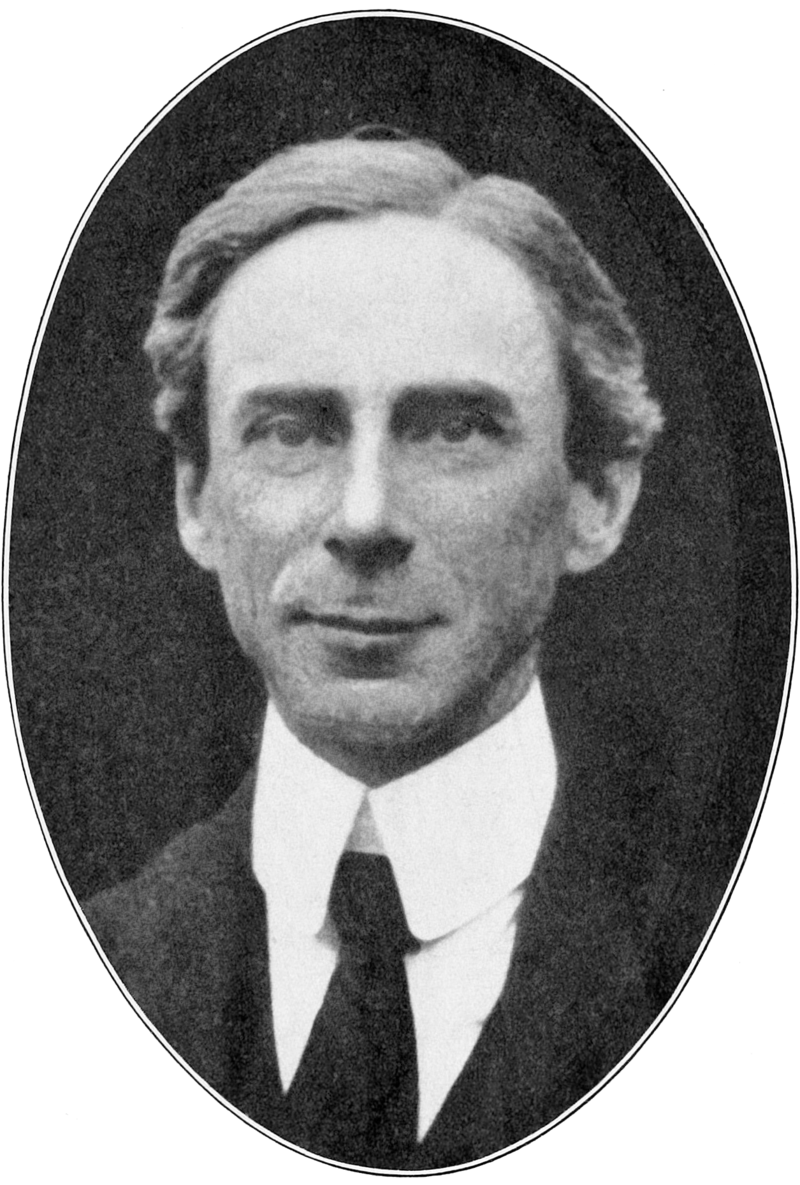
\includegraphics[width=1\textwidth]{800px-Bertrand_Russell_transparent_bg.png}\\
 				\centering
 				Bertrand~Russell \\(1872--1970)
 			\end{minipage}
 		\end{subfigure}
 	\end{figure}
 \end{frame}

 \begin{frame}{Некоторые известные языки и исчисления из математической логики}
 	\begin{itemize}
 		\item Нулевого порядка (высказываний)
 		\item Первого порядка (предикатов)
 		\item Высших порядков
 		\item Исчисление конструкций (calculus of constructions)
 	\end{itemize}
 	\begin{block}{Важное замечание}
 		То, что нельзя записать в языке, нельзя использовать в исчислениях/доказательствах
 	\end{block}
 \end{frame}

 \begin{frame}{Пример: яызк 0го порядка (высказываний) }
 	\frametitle{Знакомая вам булева (бинарная) логика}
 	\begin{figure}[t]
 		\begin{subfigure}[t]{0.45\textwidth}
 			\begin{enumerate}
 				\item Логические константы True и False
 				\item Логические переменные $x,y,z,\dots$
 				\item Бинарные связки $\vee, \wedge, \Rightarrow$ и т.д.
 			\end{enumerate}
 			\vspace{2em}
 			Правила вывода в исчислении, например:
 			\begin{mathpar}
 				\inferrule* [Right=modus ponens]
 				{ P\Rightarrow Q \\    P  }{Q}
 			\end{mathpar}
 		\end{subfigure}
 		\hspace{0.05\textwidth}
 		\begin{subfigure}[t]{0.46\textwidth}
 			\begin{theorem}[Язык и исчисление \textbf{``хорошие''}]
 				Верную формулу можно доказать за конечное число шагов. Ложную можно опровергнуть.\\

 				Т.е. существует алгоритм, который всегда завершается и говорит да/нет.
 			\end{theorem}
 			\vspace{2em}
 			Язык и исчисление \textbf{``плохие''}, потому что не всё можно записать (где кванторы?)
 		\end{subfigure}
 	\end{figure}


 \end{frame}


 \begin{frame}{Разрешимые и неразрешимые задачи}
 	\begin{definition}[Алгоритмически неразрешимая задача]
 		Задача, которая имеет ответ ``да'' или ``нет'', но для которое невозможно реализовать алгоритм, который \emph{всегда завершается, и выдает правильный ответ}.
 	\end{definition}
 	\begin{definition}[Полуразрешимая задача]
 		Неразрешимая задача, для которой можно предъявить алгоритм, который либо дает правильный ответ  ``да'', либо не завершается. Полуразрешимые$^{+}$ умеют говорить ``да'', полуразрешимые$^{-}$ --- ``нет''.
 	\end{definition}
 	Как доказывать неразрешимость
 	\begin{itemize}
 		\item Разбирать случаи и искать противоречие в каждом
 		\item Сводить каноничную неразрешимую задачу к нашей
 	\end{itemize}
 \end{frame}

 \begin{frame}{Язык и исчисление 1-го порядка (предикатов)}
 	%\framesubtitle{Вы это видели на матане}
 	\begin{figure}[t]
 		\begin{subfigure}[t]{0.5\textwidth}
 			Термы:
 			\begin{itemize}
 				\item Предметные константы: 1.0, 42, $\pi$
 				\item Функциональные символы арности  $1\leqslant n$ от термов. Например, $+, \times, f, mod$ и т.д.
 				\item Предметные переменные $x,y,z,\dots$
 			\end{itemize}
 			Формулы:
 			\begin{itemize}
 				\item Логические константы True и False
 				\item Бинарные связки $\vee, \wedge, \Rightarrow$ (и т.д.) %(от двух формул)
 				\item Предикатные символы (от термов) арности $1\leqslant n$
 				\item Кванторы $\forall, \exists$ от имени предметной переменной и формулы
 			\end{itemize}
 		\end{subfigure}
 		\hspace{0.05\textwidth}
 		\begin{subfigure}[t]{0.4\textwidth}
 			\begin{block}{Важно}
 				$+, \times, f, mod$ это названия функциональных символов, никто не гарантирует, что  $+$ это сложение чисел
 			\end{block}
 			\vspace{1em}
 			Пример: \\
 			$\forall x z\ \exists y (x < y) \wedge (y < z)$\\
 			верно, если $x,y,z \in \mathbb{R}$, \\
 			неверно, если $x,y,z \in \mathbb{N}$
 		\end{subfigure}
 	\end{figure}
 \end{frame}

 \begin{frame}{Преимущества и недостатки языка 1го порядка}

 	\begin{itemize}
 		\item Для некоторых формул из синтаксиса можно понять, что они верны (общезначимы). Для них есть алгоритм, который их докажет за конечное число шагов (см. ``метод британского музея'')
 		\item Огромное количество формул верны только в некоторой семантике, для них нельзя предъявить, алгоритм, который завершается и выдает вердикт.\\
 		В общем виде проверка формулы на истинность/ложность -- неразрешимая задача
 		\item Язык недостаточно богат. Кванторы пробегают только предметные переменные, нельзя выразить ``для любой формулы P, верно...'', например, принцип индукции
 		\[
 		\forall P.\quad P(0) \Rightarrow (\forall n . P(n) \Rightarrow P(n+1))  \Rightarrow (\forall n . P(n))
 		\]
 	\end{itemize}
 \end{frame}




 \section{Лямбды как апгрейд языка предикатов}

 \begin{frame}{Но можно попробовать вывернуться}
 	\framesubtitle{Введем специальный синтаксис}

 	\[
 	\lambda P.\quad phormula(P)
 	\]
 	Опишем принцип индукции, и применим его для $P(n)\equiv 0+\dots+n=\frac{n\cdot(n+1)}{2}$
 	\[
 	\lambda P.\quad P(0) \Rightarrow \big{(}\forall n . P(n) \Rightarrow P(n+1)\big{)}  \Rightarrow \big{(}\forall n . P(n)\big{)}
 	\]\pause
 	\[
 	\text{применение/подстановка} \mathlarger{\mathlarger{\mathlarger{\mathlarger{\Downarrow  \quad\!\!\!\!\!\!\Uparrow}}}} \text{абстракция}
 	\]

 	\begin{equation} \label{eq1}
 		\begin{split}
 			(0\equiv0) & \Rightarrow (\forall n . (0+\dots+n=\frac{n\cdot(n+1)}{2}) \Rightarrow \Big{(}0+\dots+(n+1)=\frac{(n+1)\cdot(n+2)}{2}\Big{)})  \\
 			& \Rightarrow (\forall n . 0+\dots+n=\frac{n\cdot(n+1)}{2})
 		\end{split}
 	\end{equation}
 \end{frame}



 \begin{frame}{Правила работы с новым языком $\lambda$}
 	\begin{block}{$\alpha$-эквивалентность}
 		При выборе новых имен, они не должны случайно перекрыть старые.\\
 		Предложения языка, отличающиеся только переименованием переменных, считаются ($\alpha$)эквивалентными
 	\end{block}
 	Например:  если ни $P$, ни $Q$ не встречаются в $phormula$, то $\lambda P. phormula(P)  \alphaequiv{} \lambda Q. phormula(Q) $

 	\begin{block}{$\beta$-эквивалентность}
 		Если у нас встречается $(\lambda P. phormula(P))X$, то мы можем продолжить с этим работать совершив подстановку $X$ вместо $P$ в $phormula$ (записывается как $phormula[P\mapsto X]$), т.е. заменив все свободные вхождения $P$ на $X$ внутри $phormula$.
 	\end{block}
 \end{frame}




%\section{Вопросы к экзамену}
%\begin{frame}{Вопросы к экзамену}
%\begin{itemize}
%  \item Разрешимые и неразрешимые задачи
%  \item $\lambda$-исчисление. $\alpha$ и $\beta$ правила
%  \item Нумералы Чёрча. Сложение
%  \item Рекурсия и факториал на ``пальцах''
%  \item Наследование, но оно будет ещё в других билетах
%\end{itemize}
%\end{frame}

%\section{Как писать интерпретатор на Си?}
%\begin{frame}{Дэмка на С++ (1/5): представление выражений}
%\cast
%\end{frame}
%
%\begin{frame}{Дэмка на С++ (2/5): объявление стратегии}
%\strat
%\end{frame}
%
%\begin{frame}{Дэмка на С++ (3/5): тривиальная константная стратегия}
%\nostrat
%\end{frame}
%
%\begin{frame}{Дэмка на С++ (4/5): Call-by-value}
%\cbvstrat
%\end{frame}
%\begin{frame}{Дэмка на С++ (5/5): понятие наследования}
%\inheritance
%\end{frame}